\documentclass[../main.tex]{subfiles}
\graphicspath{{\subfix{../images/}}}
\begin{document}


\section{King's rule for integration}
The King rule for integration takes advantage of the fact that area is invariant under reflection and translation. By applying it we can solve many difficult integrals.

The King rule can be written as:
\begin{equation}\label{kings1}
    \int_{a}^{b} f(x)\,dx = \int_{a}^{b} f(a+b-x)\, dx
\end{equation}

Or we can also use it this way:
\begin{equation}\label{kings2}
    \int_{a}^{b} f(x)\,dx = \frac{1}{2}\int_{a}^{b} \Bigl[f(x) + f(a+b-x)\Bigl]\, dx
\end{equation}

To see where (\ref{kings1}) comes from, consider the definite integral:
\[\int_{a}^{b} f(x)\,dx\]

\begin{figure}[h]
    \centering
    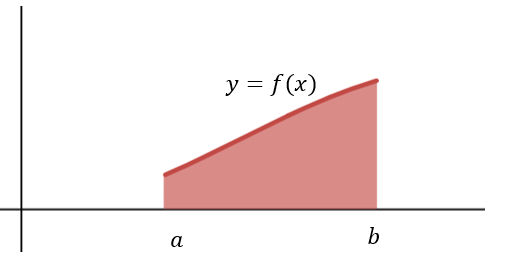
\includegraphics[width=0.4\linewidth]{images/kingsrule1.png}
\end{figure}

Firstly, let's reflect this over the y-axis. To do this, we replace {x} with {-x}, making the function $f(-x)$. Because the function is reflected in the y-axis, the upper and lower bounds on the definite integral change too. This gives us a new definite integral of:
\[\int_{-b}^{-a} f(-x)\,dx\]

\begin{figure}[h]
    \centering
    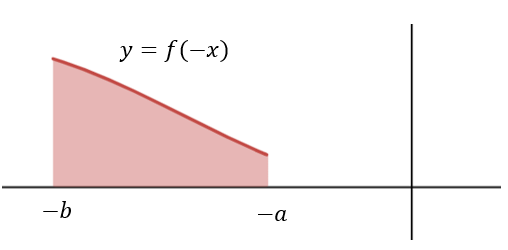
\includegraphics[width=0.4\linewidth]{images/kingsrule2.png}
\end{figure}

Next, we translate the region $a+b$ units to the right. To do this, we replace $x$ with $x-(a+b)$, making the function $f(-(x-(a+b)))$. If simplify this, the function becomes $f(a+b-x)$.

Similarly, because we are translating by $a+b$ units, the lower bound becomes $-b+(a+b)=a$ and the upper bound becomes $-a+(a+b)=b$, the same as the original integral.

This gives us a definite integral of:
\[\int_{a}^{b} f(a+b-x)\,dx\]

\begin{figure}[h]
    \centering
    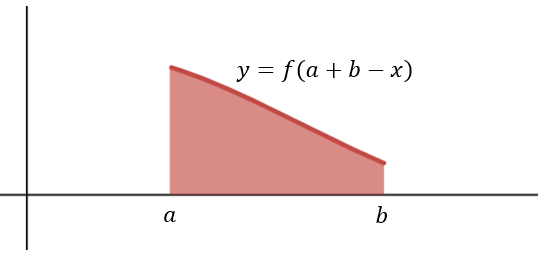
\includegraphics[width=0.4\linewidth]{images/kingsrule3.png}
\end{figure}

Since we have only reflected and translated, we know that the area of the region has not changed. In fact, we can see that the two areas will overlap with a vertical axis of symmetry at the midpoint between $a$ and $b$.

\begin{figure}[h]
    \centering
    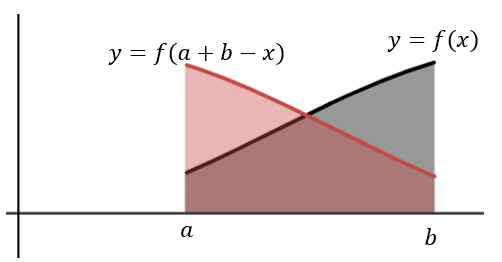
\includegraphics[width=0.4\linewidth]{images/kingsrule4.png}
\end{figure}

The second way we can apply the King rule (in (\ref{kings2}) above), can be derived by splitting the original integral into two even halves and rewriting one:
\begin{align*}
    \int_{a}^{b} f(x)\,dx &= \frac{1}{2}\int_{a}^{b} f(x)\,dx + \frac{1}{2}\int_{a}^{b} f(x)\,dx \\
    &=\frac{1}{2}\int_{a}^{b} f(x)\,dx + \frac{1}{2}\int_{a}^{b} f(a+b-x)\, dx \\
    &= \frac{1}{2}\int_{a}^{b} \Bigl[f(x) + f(a+b-x)\Bigl]\, dx
\end{align*}

So why is the King rule useful? 

Remember the following two identities based on the fact that cosine is the complement of sine:
\begin{align*}
    \sin{(\frac{\pi}{2}-\theta)}=\cos{(\theta)}\\
    \cos{(\frac{\pi}{2}-\theta)}=\sin{(\theta)}
\end{align*}

Consider the following two integrals.

\textbf{Example 1}
\[\int_0^{\frac{\pi}{2}} \sin^2{x}\,dx\]

Usually we would use a double-angle rule to rewrite $\sin^2{x}=\frac{1}{2}(1-\cos{2x})$

However, by using the second application of the King's rule the integral would go like this:

\begin{align*}
    \int_0^{\frac{\pi}{2}} \sin^2{x}\,dx &= \frac{1}{2}\int_0^{\frac{\pi}{2}}\sin^2{x}+\sin^2{\Bigl(\frac{\pi}{2}-x\Bigr)}\,dx\\
    &= \frac{1}{2}\int_0^{\frac{\pi}{2}}\sin^2{x}+\cos^2{x}\,dx \\
    &=\frac{1}{2}\int_0^{\frac{\pi}{2}}1\,dx\\
    &=\frac{1}{2}\times \Bigl[x\Bigr]_0^{\frac{\pi}{2}}\\
    &=\frac{1}{2}\times \frac{\pi}{2}=\frac{\pi}{4}
\end{align*}

\textbf{Example 2}
\begin{align*}
    \int_0^{\frac{\pi}{2}} \frac{\sin{x}}{\sin{x}+\cos{x}}\,dx &= \frac{1}{2}\int_0^{\frac{\pi}{2}}\frac{\sin{x}}{\sin{x}+\cos{x}}+\frac{\sin{(\frac{\pi}{2}-x)}}{\sin{(\frac{\pi}{2}-x)}+\cos{(\frac{\pi}{2}-x)}}\,dx\\
    &=\frac{1}{2}\int_0^{\frac{\pi}{2}}\frac{\sin{x}}{\sin{x}+\cos{x}}+\frac{\cos{x}}{\cos{x}+\sin{x}}\,dx\\
    &=\frac{1}{2}\int_0^{\frac{\pi}{2}}\frac{\sin{x}+\cos{x}}{\sin{x}+\cos{x}}\,dx\\
    &=\frac{1}{2}\times \int_0^{\frac{\pi}{2}}1\,dx\\
    &=\frac{1}{2}\times \Bigl[x\Bigr]_0^{\frac{\pi}{2}}\\
    &=\frac{1}{2}\times \frac{\pi}{2}=\frac{\pi}{4}
\end{align*}

\pagebreak
\subsection*{Questions} 
\label{Kings rule}
(Answers - page {\pageref{Kings rule answers}})

Use the King Rule to evaluate the following definite integrals:

\begin{enumerate}[itemsep=0.7cm]
    \item 
    $\int_0^{\frac{\pi}{2}}\frac{\sin^n{(x)}}{\sin^n{(x)}+\cos^n{(x)}}\,dx$

    \item 
    $\int_0^{\frac{\pi}{2}}\frac{1}{1+(\tan{x})^{\pi}}\,dx$

    \item 
    $\int_0^1 \frac{\ln{(x+1)}}{x^2+1}\,dx$

    \item 
    $\int_0^{\pi} \frac{x\sin{x}}{1+\sin{x}}\,dx$


\end{enumerate}


\pagebreak


\end{document}